\documentclass[a4paper,12pt]{extarticle}
\usepackage[utf8]{inputenc}
%\usepackage[hungarian]{babel}
\usepackage[table,xcdraw]{xcolor}
\usepackage{physics}
\usepackage{fancyhdr}
\usepackage{geometry}
\usepackage{natbib}
\usepackage{graphicx}
\usepackage{float}
\usepackage{wrapfig}
%\usepackage{caption}
\usepackage[justification=centering]{caption}
\usepackage{subcaption}
\usepackage{gensymb}
\usepackage[export]{adjustbox}
\usepackage{hyperref}
\geometry{margin = 20mm}
\usepackage{mathtools}
\usepackage{amsmath}
\usepackage{indentfirst}
\usepackage{xurl}
\usepackage{t1enc}
\usepackage{setspace}


\title{Geant4 report 1}
\author{Bendegúz Borkovits T7UR9P}
\date{February 2022}


\begin{document}
\onehalfspacing

\maketitle

\begin{center}

\includegraphics[scale=0.3]{elte_cimer_szines.jpg}

\vspace{2 cm}
Scientific Data Analytics and Modeling specialization

Scientific Modeling Computer Laboratory

Supervisor: Ákos Horváth


\end{center}

\section{Introduction}
Geant4 is a widely known Nuclear and Particle physics software package and with it, it is possible to model the process of detecting many different particles with the usage of a simulated detector. The aim of this project is to become familiar with the mentioned software and use it to simulate a given physical system that includes modeling a specific type of detector.

\section{Installation and testing}

For the first week, the task was to install Geant4 and test its visualization using its input files. To provide the suitable environment for the software, I installed Windows Subsystem for Linux and Xming, however Geant4 could not function with these tools. Therefore, I installed Oracle VM VirtualBox and created a virtual Ubuntu 20.04 virtual machine. After testing, it turned out that one should use an older version of VirtualBox, since apparently the newest one seems to be unstable.

After setting up the environments, I installed and built Geant4 with cmake and tested it by building and running one of the simpler examples the software package offered. The visualization tool successfully showed the result of the simulation, thus confirming, that everything went well during installation. It should be noted that the geant4make.sh file needs to be sourced each time a user newly opens up Geant4 or the presence of one of the graphical libraries will not register and the program will refuse to run.

\begin{figure}[H]
    \centering
    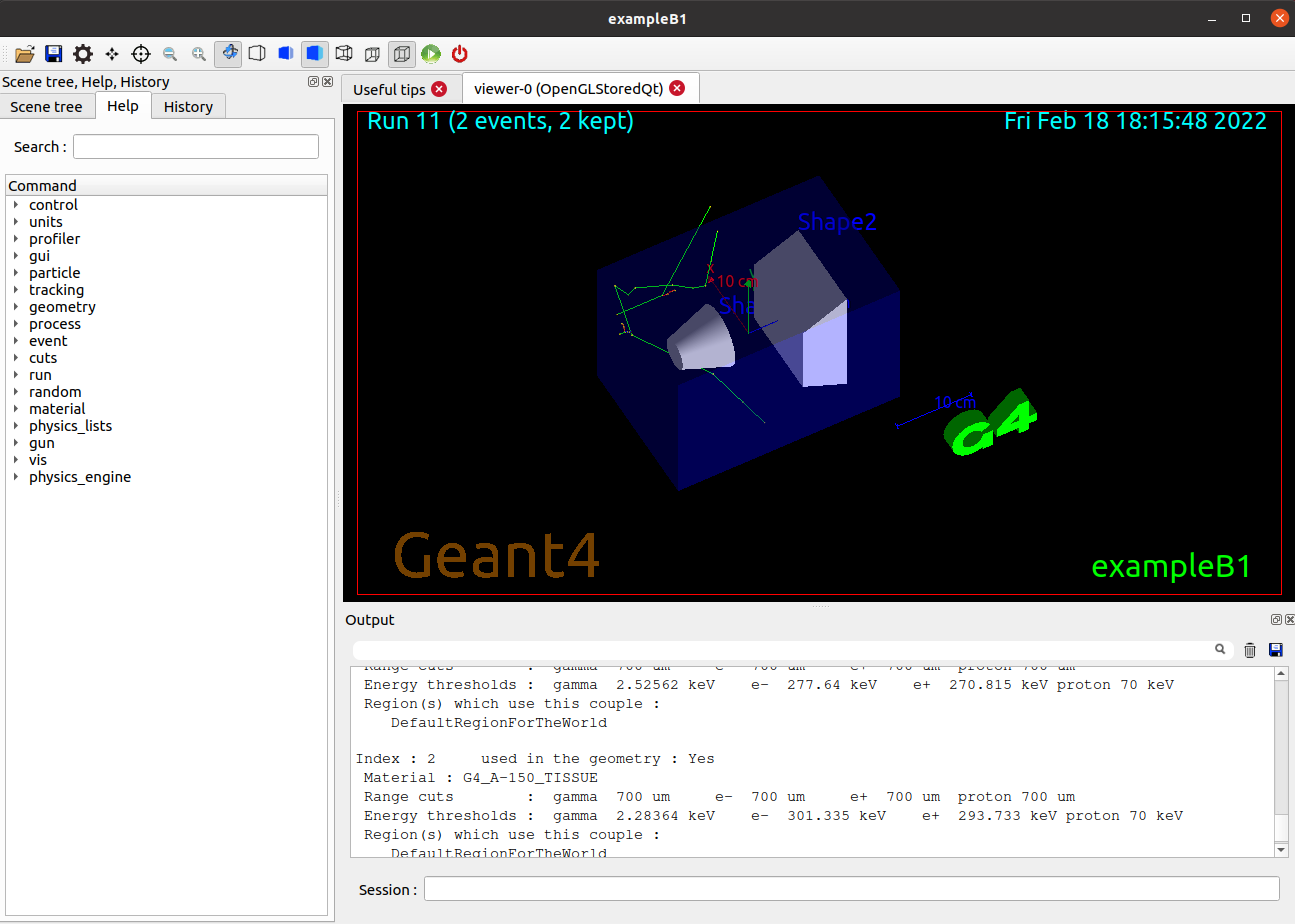
\includegraphics[scale=0.5]{geantkep.png}
    \caption{The example program B1 with the erratic green lines representing two particles.}
\end{figure}

\section{References}
\begin{itemize}
    \item Oracle VM VirtualBox: \url{https://www.virtualbox.org/wiki/Downloads}
    \item Ubuntu 20.04: \url{https://ubuntu.com/download/desktop}
    \item Geant4: \url{https://geant4.web.cern.ch/support/download}
\end{itemize}



\end{document}
